\documentclass[a4paper,12pt]{article}

% Mise en page
\textwidth 18cm
\textheight 26cm 
\topmargin -2 cm 
\oddsidemargin -1cm 
\evensidemargin -1cm
% \renewcommand{\baselinestretch}{1.1}  

% Texte
%\usepackage[french]{babel}
\usepackage[latin1]{inputenc}
\usepackage{amsmath, amssymb, amsfonts, stmaryrd}
\usepackage{enumerate}
\usepackage{xcolor}
\usepackage{graphicx}
\usepackage{xspace}
\usepackage{/home/robin/LATEX/Biblio/astats}

% Commande
\newcommand{\Bcal}{\mathcal{B}}
\newcommand{\BM}{\text{BM}}
\newcommand{\Cov}{\mathbb{C}\text{ov}}
\newcommand{\dd}{\text{d}}
\newcommand{\Ecal}{\mathcal{E}}
\newcommand{\Esp}{\mathbb{E}}
\newcommand{\Gcal}{\mathcal{G}}
\newcommand{\Ibb}{\mathbb{I}}
\newcommand{\Ncal}{\mathcal{N}}
\newcommand{\OU}{\text{OU}}
\newcommand{\Pbb}{\mathbb{P}}
\newcommand{\ra}{$\rightarrow$ \xspace}

%%%%%%%%%%%%%%%%%%%%%%%%%%%%%%%%%%%%%%%%%%%%%%%%%%%%%%%%%%%%%%%%%%%%%%
%%%%%%%%%%%%%%%%%%%%%%%%%%%%%%%%%%%%%%%%%%%%%%%%%%%%%%%%%%%%%%%%%%%%%
\begin{document}
%%%%%%%%%%%%%%%%%%%%%%%%%%%%%%%%%%%%%%%%%%%%%%%%%%%%%%%%%%%%%%%%%%%%%%
%%%%%%%%%%%%%%%%%%%%%%%%%%%%%%%%%%%%%%%%%%%%%%%%%%%%%%%%%%%%%%%%%%%%%%

\title{Recurrent genomic alterations and excursions of Markovian processes}
\author{S. Robin \\
  ~\\
  \begin{tabular}{lp{0.8\textwidth}}
   Joint work with:    & V. Stefanov (Sections \ref{sec:np} and \ref{sec:Np}) \\
   & L. Decreusefond, M.-P. Etienne, G. Lang, P. Vallois (Section \ref{sec:NP}).
  \end{tabular}
} 
\date{\today}
\maketitle

\tableofcontents

%%%%%%%%%%%%%%%%%%%%%%%%%%%%%%%%%%%%%%%%%%%%%%%%%%%%%%%%%%%%%%%%%%%%%%
%%%%%%%%%%%%%%%%%%%%%%%%%%%%%%%%%%%%%%%%%%%%%%%%%%%%%%%%%%%%%%%%%%%%%%
\newpage
\section{Problem}
%%%%%%%%%%%%%%%%%%%%%%%%%%%%%%%%%%%%%%%%%%%%%%%%%%%%%%%%%%%%%%%%%%%%%%

%%%%%%%%%%%%%%%%%%%%%%%%%%%%%%%%%%%%%%%%%%%%%%%%%%%%%%%%%%%%%%%%%%%%%%
\subsection{Genomic alterations} 

$$
\text{\textcolor{red}{\sl See slides.}}
$$

%%%%%%%%%%%%%%%%%%%%%%%%%%%%%%%%%%%%%%%%%%%%%%%%%%%%%%%%%%%%%%%%%%%%%%
\subsection{Problem}
\paragraph{Data.} 
\begin{itemize}
  \item $p$ patients: $i = 1..p$;
  \item $n$ loci: $t = 1..n$;
  \item $X_i =$ profile of patient $i$:
  $$
  X_i(t) = \left\{\begin{array}{ll}
  1 & \text{if patient $i$ altered at locus $t$,} \\
  0 & \text{otherwise.}
  \end{array}\right.
  $$
\end{itemize}

\paragraph{Cumulated profile.}
$$
S_p(t) = \sum_{i=1}^p X_i(t) = \text{number of patients carrying an alteration at locus $t$}.
$$

%%%%%%%%%%%%%%%%%%%%%%%%%%%%%%%%%%%%%%%%%%%%%%%%%%%%%%%%%%%%%%%%%%%%%%
\subsection{Generic model}
\paragraph{Null model.} $\{X_i\}_i$ iid homogeneous Markov processes
$$
\text{homogeneity } \rightarrow \text{ no preferential region for alterations}.
$$
{\sl Because the $X_i$ are both Markov, binary and iid, $S_p$ is still Markovian (see later).}

\paragraph{Significance.}
\begin{eqnarray*}
\pi(m, \ell) & = & \Pr\{\text{$S_p$ has one an excursion above $m$ longer than $\ell$}\} \\
& = & \Pr\{\exists \ell \leq t \leq n, \forall t-\ell < s \leq t: S_p(s) \leq m\}
\end{eqnarray*}
also depends on $n$, $p$ and the common parameters of the processes $X_i$, namely $\lambda$ and $\mu$ (see later).

%%%%%%%%%%%%%%%%%%%%%%%%%%%%%%%%%%%%%%%%%%%%%%%%%%%%%%%%%%%%%%%%%%%%%%
%%%%%%%%%%%%%%%%%%%%%%%%%%%%%%%%%%%%%%%%%%%%%%%%%%%%%%%%%%%%%%%%%%%%%%
\newpage
\section{CGH BAC arrays: small $p$, small $n$ \label{sec:np}}
%%%%%%%%%%%%%%%%%%%%%%%%%%%%%%%%%%%%%%%%%%%%%%%%%%%%%%%%%%%%%%%%%%%%%%

\paragraph{Long time ago:} $n \simeq 10^2$, $p \simeq 10^{1-2}$ 

%%%%%%%%%%%%%%%%%%%%%%%%%%%%%%%%%%%%%%%%%%%%%%%%%%%%%%%%%%%%%%%%%%%%%%
\subsection{Model}

\paragraph{Model for an individual profile.} $X_i = \{X_i(t)\}_{t = 1..n} =$ discrete time Markov chain with two states:
$$
X_i \sim MC(\nu, P)
$$
where $\nu = $ initial distribution (e.g. stationary distribution) and $P =$ transition matrix:
$$
P = 
\left( \begin{array}{cc}
  1-\lambda & \lambda \\
    \mu & 1 - \mu
\end{array} \right)
$$
Interpretation: 
\begin{itemize}
 \item $1/\mu =$ mean alteration length, 
 \item $n\lambda\mu/(\lambda+\mu) =$ mean number of alterations per patient.
\end{itemize}

\paragraph{Model for the cumulated profile.} As the $X_i$'s are Markovian, binary and iid, we have
\begin{eqnarray*}
  \Pr\{S_p(t+1) = b | \{X_i(s)\}_{1 \leq i \leq n; s\leq t}\} & = & \Pr\{S_p(t+1) = b | \{X_i(t)\}_{1 \leq i \leq n}\} \\
  & = & \sum_{c=0}^b \binom{S_p(t)}{c} (1-\mu)^c \mu^{S_p(t) - c} \binom{n-S_p(t)}{b-c} \lambda^{b-c} (1-\lambda)^{n - S_p(t) - b + c} \\
  & = & \Pr\{S_p(t+1) = b | S_p(t)\}
\end{eqnarray*}
so $S_p$ is an homogeneous Markov chain with transition
$$
\left(S_p(t+1) | S_p(t) = a\right) \overset{\Delta}= \Bcal(a, 1-\lambda) + \Bcal(n-a, \mu).
$$
Let $P_S$ denote its transition matrix:
$$
[P_S]_{ab} = \Pr\{S_p(t+1) =b | S_p(t) = a\} := \sum_{c=0}^b \binom{a}{c} (1-\mu)^c \mu^{a - c} \binom{n-a}{b-c} \lambda^{b-c} (1-\lambda)^{n - a - b + c} .
$$
Its initial distribution $\nu_S$ can be established in the same way.

%%%%%%%%%%%%%%%%%%%%%%%%%%%%%%%%%%%%%%%%%%%%%%%%%%%%%%%%%%%%%%%%%%%%%%
\subsection{Embedded Markov chain}
$P_S$ describes the transition of $S_p$ but not directly is excursions above $m$ \ra not easy to compute $\pi(m, \ell)$.

\paragraph{Principle of embedded Markov chain:} Construct a surrogate MC, such that the event of interest
$$
\{\text{an excursion above $m$ with length $\ell$ occurs}\}
$$
is an absorbing state.

\paragraph{Construction of the embedded Markov chain.} 
$$
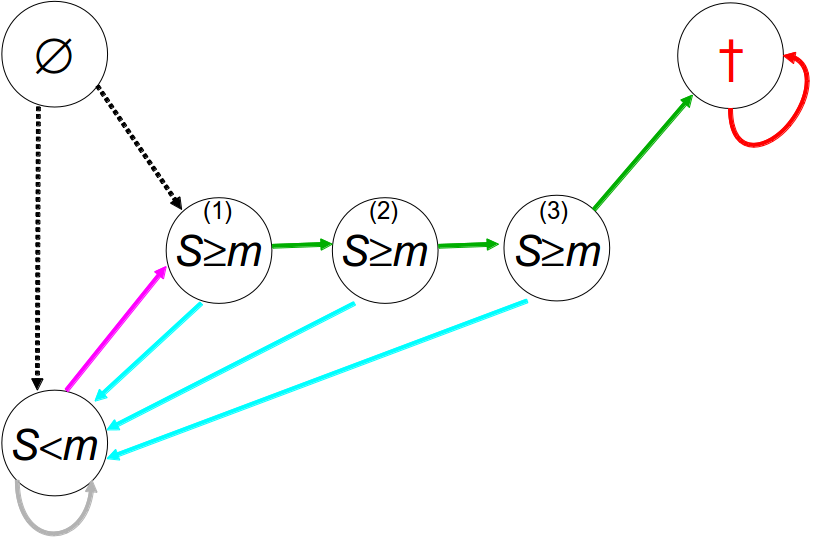
\includegraphics[width=.3\textwidth, clip=]{../FIGURES/Fig-MinReg-Automaton}
$$
Relabel $p+1$ states
$$
0, 1, \dots, m-1, m, \dots, p
$$
into $m + (\ell-1)(p-m+1) + 1$
$$
0, 1, \dots, m-1, \underset{\text{First time above $m$}}{\underbrace{m^{(1)}, \dots, p^{(1)}}}, \dots , \underset{\text{$\ell-1$-th time above $m$}}{\underbrace{m^{(\ell-1=}, \dots, p^{(\ell-1)}}}, \dagger
$$
where $\dagger$ stands for the 'coffin' (absorbing) state, and construct the corresponding transition matrix $\widetilde{P}_S = \widetilde{P}_S(m, \ell)$:
$$
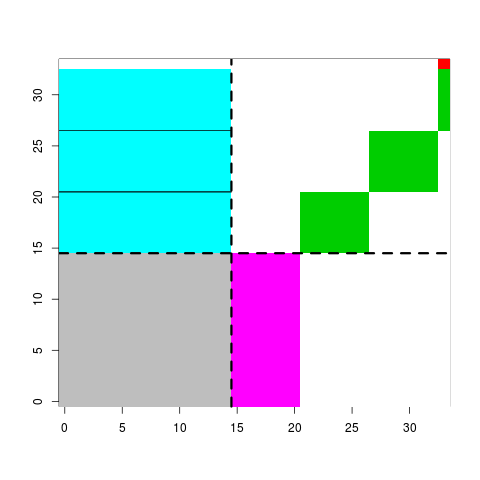
\includegraphics[width=.5\textwidth]{../FIGURES/Fig-MinReg-EmbMC-Abs} \\
$$
and its initial distribution similarly:
$$
\widetilde{\nu}_S = [\nu_S^\intercal \; 0 \; \dots \; 0].
$$
%%%%%%%%%%%%%%%%%%%%%%%%%%%%%%%%%%%%%%%%%%%%%%%%%%%%%%%%%%%%%%%%%%%%%%
\subsection{Significance}
We simply need to compute
$$
\pi(m, \ell) = \left[\widetilde{\nu}_S^\intercal \left(\widetilde{P}_S\right)^{n-1}\right]_\dagger
$$

%%%%%%%%%%%%%%%%%%%%%%%%%%%%%%%%%%%%%%%%%%%%%%%%%%%%%%%%%%%%%%%%%%%%%%
%%%%%%%%%%%%%%%%%%%%%%%%%%%%%%%%%%%%%%%%%%%%%%%%%%%%%%%%%%%%%%%%%%%%%%
\newpage
\section{SNP arrays: small $p$, large $n$ \label{sec:Np}}

\paragraph{Not that long ago:} $n \simeq 10^{4-5}$, $p \simeq 10^{1-2}$


%%%%%%%%%%%%%%%%%%%%%%%%%%%%%%%%%%%%%%%%%%%%%%%%%%%%%%%%%%%%%%%%%%%%%%
\subsection{Model}

\paragraph{Model for an individual profile.} $X_i = \{X_i(t)\}_{0 \leq t \leq n} =$ and the $X_i$'s are iid {\sl continuous-time} Markovian binary process with rates
\begin{equation} \label{Eq:XiBD}
\begin{array}{lll}
\text{alteration 'birth'} & 0 \rightarrow 1: & \lambda \\
\text{alteration 'death'} & 1 \rightarrow 0: & \mu
\end{array}
\end{equation}
which means that 
\begin{itemize}
 \item the alteration length are $\Ecal(\mu)$ and 
 \item the normal regions between alteration have length $\Ecal(\lambda)$.
\end{itemize}

\paragraph{Model for the cumulated profile.} For the same reason as before, $S_p = \{S_p(t)\}_{0 \leq t \leq n}$ is a continuous-time Markov process over $\{0, \dots p\}$, known as 'birth \& death' process with rates
$$
\begin{array}{llrcl}
  \text{alteration 'birth'} & s \rightarrow s+1: & \lambda_s & = & \lambda \times (p-s)\\
  \text{alteration 'death'} & s \rightarrow s-1: & \mu_s & = & \mu \times s
\end{array}
$$
that is, with the $(p+1) \times (p+1)$ generator 
$$
Q_S = \left(
  \begin{array}{cccccccc}
   \square & \lambda p \\
   \mu & \square & \lambda (p-1) \\
   & \ddots & \ddots & \ddots & \\
   & & \mu s & \square & \lambda (p-s) \\
   & & & \ddots & \ddots & \ddots & \\
   & & & & \mu (p-1) & \square & \lambda \\
   & & & & & \mu p & \square \\
  \end{array}
\right)
$$
where the diagonal terms $\square$ are such that the sum of each row is 0. This generator is also called transition kernel as
$$
\Pr\{S_p(t+s) = b \;|\; S_p(t) = a\} = \left[e^{s Q_S}\right]_{a, b}.
$$

%%%%%%%%%%%%%%%%%%%%%%%%%%%%%%%%%%%%%%%%%%%%%%%%%%%%%%%%%%%%%%%%%%%%%%
\subsection{Probability generating function}

\paragraph{Definition of the waiting time.} Define
$$
T(m, \ell) = \inf\{\ell < t \leq n: \forall t-\ell < s \leq t, S_p(s) \leq m \},
$$
we have that
$$
\pi(m, \ell) = \Pr\{T \leq n\}
$$
\ra $\pi(m, \ell)$ is given by the distribution of $T(m, \ell)$.

\paragraph{Construction of the waiting time.}
Defining a generic hitting time as 
$$
H_{a \rightarrow b} = \inf\{t \geq 0: S_p(t) = b \;|\; S_p(0) = a\}
$$
and further define
$$
A := H_{S_p(0) \rightarrow m}, 
\qquad
B := H_{(m \rightarrow m-1 \;|\; < \ell)}, 
\qquad
C := H_{m-1 \rightarrow m},
$$
we have that
\begin{equation} \label{Eq:Tml}
T(m, \ell) = A + \sum_{g=1}^G (B_g + C_g) + \ell
\end{equation}
where $\{B_g\}$ and $\{C_g\}$ are iid copies of $B$ and $C$, respectively, and $G$ is a geometric rv with success probability $\gamma = \Pr\{H_{m \rightarrow m-1} \geq \ell\}$.
$$
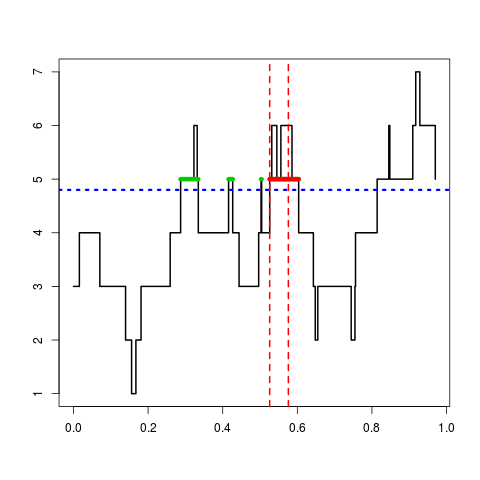
\includegraphics[height=.5\textwidth, width=.7\textwidth]{../FIGURES/Fig-MinReg-BirDea-OK} 
$$

%%%%%%%%%%%%%%%%%%%%%%%%%%%%%%%%%%%%%%%%%%%%%%%%%%%%%%%%%%%%%%%%%%%%%%
\subsection{Significance}

\paragraph{A reminder on probability generating function (pgf).} For a non-negative rv $H$, define
$$
\phi_H(x) = \Esp(x^H), 
$$
we have the following properties\footnote{Geometric distribution: in a sequence of independent trials: number of failure before a success, which occurs with probability $p$.}
\begin{eqnarray*}
 U \perp V & \Rightarrow & \phi_{U+V}(x) = \phi_U(x) \phi_V(x), \\
 (U_i) \text{ iid } \perp V (\text{integer}) & \Rightarrow & \phi_V\left[\phi_U(x)\right], \\
 U \text{ geometric } \Gcal(p) & \Rightarrow & \phi_U(x) = p \left/ \left[1 - (1-p)x\right] \right..
\end{eqnarray*}

\paragraph{Pgf of $T(m, \ell)$.} Because $S_p$ is Markovian, it is a renewal process (which means that all the successive hitting times $A, B_1, C_1, \dots,  B_G, C_G$ are independent), so \eqref{Eq:Tml} yields
\begin{eqnarray*}
  \phi_T(x) 
  & = &  \phi_A(x) \; \phi_{\sum_{g=1}^G (B_g + C_g)}(x) x^\ell 
  \; = \; \phi_A(x) \; \phi_G \left[\phi_{B+C}(x)\right] x^\ell \\
  & = & \phi_A(x) \; \phi_G[\phi_B(x) \phi_C(x)] \; x^\ell 
  \; = \; \frac{\gamma \; \phi_A(x) \; x^\ell}{1 - (1 - \gamma) [\phi_B(x) \phi_C(x)]}.
\end{eqnarray*}
\cite{BaS01} provide the Laplace transform $\psi_H(x) = \phi_H(e^{-x})$ of any hitting time of a finite birth \& death process with linear rates. \\
\ra $\psi_A$, $\psi_B$ and $\psi_C$ are known. \\
\ra The Laplace transform $\psi_T(x)$ of $T(m, \ell)$ can be derived in a similar way. \\
\ra Its cumulative Laplace transform $\Psi_T(x)$ follows.

\paragraph{In practice.} Need to invert $\Psi_T(x)$ using, e.g. \cite{AbW06}:
$$
\text{\ra strong numerical instabilities}
$$
%%%%%%%%%%%%%%%%%%%%%%%%%%%%%%%%%%%%%%%%%%%%%%%%%%%%%%%%%%%%%%%%%%%%%%
%%%%%%%%%%%%%%%%%%%%%%%%%%%%%%%%%%%%%%%%%%%%%%%%%%%%%%%%%%%%%%%%%%%%%%
\newpage
\section{DNAseq: large $p$, large $n$  \label{sec:NP}}
\newcommand{\St}{\widetilde{S}}
\newcommand{\Tt}{\widetilde{T}}
\newcommand{\mt}{\widetilde{m}}

\paragraph{Today:} $n \simeq 10^{6-8}$, $p \simeq 10^{3-4}$

%%%%%%%%%%%%%%%%%%%%%%%%%%%%%%%%%%%%%%%%%%%%%%%%%%%%%%%%%%%%%%%%%%%%%%
\subsection{Model}

\paragraph{Model for an individual profile.} Same Model \eqref{Eq:XiBD} as for the small $p$, large $n$ case.

\paragraph{Model for the cumulated profile.} Same setting, but letting $p$ grow to infinity. Define the normalized process:
$$
\St_p(t) := \frac{S_p(t) - p \theta}{\sigma \sqrt{p}}. 
$$
where $\tau = \lambda + \mu$, $\theta = \lambda/\tau$, $\sigma^2 = \theta(1-\theta)$. In the stationary regime:
$$
S_p(t) \sim \Bcal(p, \theta) 
\qquad \Rightarrow \qquad 
\St_p(t) \underset{p \rightarrow \infty}{\overset{\Delta}{\longrightarrow}} \Ncal(p \theta, p \sigma^2).
$$
One can show in the same way that all finite-dimensional marginals of $\St$ are asymptotically Gaussian, so $\St$ is a Gaussian process with covariance kernel
$$
\Cov\left[\St(t), \St(t+s)\right] = e^{-\tau s}
$$
so we recognize a Ornstein-Uhlenbeck process:
$$
\St_p \underset{p \rightarrow \infty}{\overset{\Delta}{\longrightarrow}} \OU(\tau).
$$
Remind that an $\OU(\tau)$ process $Z$ satisfies the stochastic differential equation:
$$
\dd Z(t) = - \tau Z(t) + \dd B(t)
$$
where $B(t)$ is the standard Brownian motion ($\BM$). 
$$
\text{\ra $Z(t)$ is both a continuous-time and continuous-state Markov process.}
$$

%%%%%%%%%%%%%%%%%%%%%%%%%%%%%%%%%%%%%%%%%%%%%%%%%%%%%%%%%%%%%%%%%%%%%%
\subsection{Excursions}

In this setting, the limit of $\pi(m, \ell)$ as $p$ grows to infinity can be rephrased as
\begin{eqnarray*}
\lim_{p \rightarrow \infty} \pi(m, \ell) 
& = & \Pr\{\text{the longest excursion of $Z(t)$ above $\mt$ exceeds $\ell$}\} \\
& = & \Pr\{\max_{\ell < t \leq n} \St^{-\ell}(t) \geq \mt\}
\end{eqnarray*}
where $\mt = (m - p \theta)/\sigma \sqrt{p}$ and $\St^{-\ell}(t) = \min_{t-\ell < s \leq t} \St(s).$

\paragraph{Convergence of $\pi(m,  \ell)$.} Because $\max_{\ell < t \leq n} \St^{-\ell}(t)$ is a continuous transform of the process $S_p$, the convergence in distribution of $\St_p$ toward an $OU$ process ensures that the probability of interest $\pi(m, \ell)$ for $\St_p$ also converges toward the same quantity for the limit $OU$ process.

% \paragraph{$\OU$ hitting times.} 

\paragraph{Brownian excursions.} Very few is known about the excursions of an $\OU$ process above an arbitrary threshold. \cite{PiY97} provide a simple way to sample the lengths 
$$
V_{(1)} \geq V_{(2)} \geq \dots
$$
(and their signs) of a Brownian motion apart from 0.

%%%%%%%%%%%%%%%%%%%%%%%%%%%%%%%%%%%%%%%%%%%%%%%%%%%%%%%%%%%%%%%%%%%%%%
\subsection{Significance}

% \paragraph{Waiting time.} $\pi(m, \ell)$ can also be defined via a hitting time:
% $$
% \Tt = \inf\{t>\ell: \St^{-\ell}(t) \geq \mt\}.
% $$

\paragraph{Girsanov formula.} Letting aside (a lot of non-trivial) technicalities, we have that
$$
\frac{\dd \Pbb_{\OU}}{\dd \Pbb_{\BM}} = w(\{V_{(k)}\}_{k \geq 1}, ...)
$$

\paragraph{Monte-Carlo estimation.} $\pi(m, \ell)$ can be estimated with an arbitrary precision via Monte-Carlo in the following way. First note that
$$
\pi(m, \ell) = \Esp[g(Z)]
$$
where 
$$
g(Z) = \Ibb\{\text{the longest excursion of $Z$ above $\mt$ exceeds $\ell$}\}.
$$
Then, one can simply sample a (large number) $B$ if independent paths of $\{Z(t)\}_{0 \leq t \leq n}$ and estimate $\pi(m, \ell)$ as
$$
\widehat{\pi}(m, \ell) = \frac1B \sum_b g(Z^b).
$$
\ra This requires to sample whole (continuous) paths of $Z$.

\paragraph{Importance sampling.} Suppose we are interested in the evaluation of $\Esp[g(Z)]$, while not being able to sample from $Z$, but only from another rv $Y$. First note that
$$
\Esp[g(Z)] = \int g(z) \dd \Pbb_Z(z) = \int g(y) \underset{w(y)}{\underbrace{\frac{\dd \Pbb_Z(y)}{\dd \Pbb_Y(y)}}} \dd \Pbb_Y(y)
$$
provided that $\Pbb_Y \gg \Pbb_Z$. Then, one can sample a large number of $Y$ and estimated $\Esp[g(Z)]$ as
$$
\widehat{\Esp}[g(Z)] = \frac1{\sum_b w(y^b)} \sum_b g(y^b) w(y^b). 
$$

\paragraph{Back to significance.} The importance sampling scheme applies for $Z \sim \OU$ and $Y \sim \BM$. Because both $g(y)$ and $w(y)$ (almost) only relies on the $V_{(k)}$'s, this does not require to sample whole Brownian motion paths.

%%%%%%%%%%%%%%%%%%%%%%%%%%%%%%%%%%%%%%%%%%%%%%%%%%%%%%%%%%%%%%%%%%%%%%
%%%%%%%%%%%%%%%%%%%%%%%%%%%%%%%%%%%%%%%%%%%%%%%%%%%%%%%%%%%%%%%%%%%%%%
\newpage
\section{Appendix}
%%%%%%%%%%%%%%%%%%%%%%%%%%%%%%%%%%%%%%%%%%%%%%%%%%%%%%%%%%%%%%%%%%%%%%

%%%%%%%%%%%%%%%%%%%%%%%%%%%%%%%%%%%%%%%%%%%%%%%%%%%%%%%%%%%%%%%%%%%%%%
\subsection{Some proofs}

\paragraph{Proofs for pgf properties.}
$$
\phi_{\sum_{i=1}^V U_i}(x) = \Esp_V \Esp_{(U_i)}\left[x^{\sum_{i=1}^V U_i} \;|\; V\right] 
 = \Esp_V \left[\phi_U(x)^V\right] 
 = \phi_V\left[\phi_U(x)\right].
$$
$U$ geometric:
$$
\phi_U(x) = \sum_{u \geq 0} (1-p)^u p x^u 
= p \sum_{u \geq 0} [x(1-p)]^u 
= \frac{p}{1 - (1-p)x}.
$$

\paragraph{Laplace transform.} For a positive rv, define
$$
\psi_U(x) = \Esp(e^{-xU}) = \phi_U(e^{-x}) = \int f(u) e^{-xu} \dd u
$$
and its counterpart for the cdf:
$$
\Psi_U(x) = \int F(u) e^{-xu} \dd u.
$$
We have
$$
\Psi_U(x) = \left[ - \frac1x F(u) e^{-xu}\right]_0^\infty - \left(-\frac1x\right) \int f(u) e^{-xu} \dd u = \frac{\phi_U(x)}x.
$$

% \paragraph{Pgf of the survival.}
% Denote $\Phi_U(x) = \int_0^\infty S(u) x^u \dd u$ where $S$ is the survival function $S(u) = \int_u^\infty f(u) \dd u$. Because 
% $$
% S(\infty) = 0, 
% \quad
% \frac{\partial S(u)}{\partial u} = -f(u), 
% \quad 
% \frac{\partial x^u}{\partial u} = x ^u \log x,
% $$
% we have
% $$
% \Phi_U(x) = \int_0^\infty S(u) x^u \dd u 
% = \left[\frac{S(u) x^u}{\log x} \right]_0^\infty - \int_0^\infty [-f(u)] \frac{x^u}{\log x} \dd u
% = \frac{\phi_U(x)}{\log x}.
% $$

%%%%%%%%%%%%%%%%%%%%%%%%%%%%%%%%%%%%%%%%%%%%%%%%%%%%%%%%%%%%%%%%%%%%%%
%%%%%%%%%%%%%%%%%%%%%%%%%%%%%%%%%%%%%%%%%%%%%%%%%%%%%%%%%%%%%%%%%%%%%%
% \newpage
\bigskip
\bibliographystyle{/home/robin/LATEX/Biblio/astats}
\bibliography{/home/robin/Biblio/AST,/home/robin/Biblio/ARC,/home/robin/Biblio/SSB}

%%%%%%%%%%%%%%%%%%%%%%%%%%%%%%%%%%%%%%%%%%%%%%%%%%%%%%%%%%%%%%%%%%%%%%
%%%%%%%%%%%%%%%%%%%%%%%%%%%%%%%%%%%%%%%%%%%%%%%%%%%%%%%%%%%%%%%%%%%%%%
\end{document}
%%%%%%%%%%%%%%%%%%%%%%%%%%%%%%%%%%%%%%%%%%%%%%%%%%%%%%%%%%%%%%%%%%%%%%
%%%%%%%%%%%%%%%%%%%%%%%%%%%%%%%%%%%%%%%%%%%%%%%%%%%%%%%%%%%%%%%%%%%%%%


